\section{}
\textbf{Proof for $\bf{N_2^1\| P_2\| N_2^2\preceq_t N_3^1\| P_3\| N_3^2}$}\\\\
In this subsection we manually prove the timed simulation relation $N_2^1\| P_2\| N_2^2\preceq_t N_3^1\| P_3\| N_3^2$. The other relations can be proved accordingly.
\subsection{Timed Simulation Relation \textsf{sim}}
For two timed automata $T^1$ and $T^2$, we write timed simulation relation \textsf{sim} is defined on $\Omega_1\times\Omega_2$ where $(s,v)\in\Omega_1$ and $v$ is the valuation of all clocks $t_1\in X_1$. $((s,v),(s',v'))$ is in \textsf{sim} if and only if $v'=v(\lambda+\delta)$, for $\delta\in D$, such that \textsf{sim}$(s,v)=(s',v(\lambda +D))$

%There exists $d\in D$ such that $(s',v(t+d))\in\Omega_2$
Let $T^1=N_2^1\| P_2\| N_2^2$ and $T^2=N_3^1\| P_3\| N_3^2$. $X_1=\{tn_2^1,tp_2,tn_2^2\}$ and $X_2=\{tn_3^1,tp_3,tn_3^2\}$, the state mapping for the timed simulation relation is shown below:\\
\\
\textsf{sim}($RE\| ID\| RE,v)=(RE\| ID\| RE,v(tn_3^1+D_1,tn_3^2+D_2)$)
where $D_1=[N_2^1.Terp\_min,N_2^1.Terp\_max]$,\\
 $D_2=[N_2^2.Terp\_min,N_2^2.Terp\_max]$\\
\\
A special condition for this mapping is the initial state:\\
\textsf{sim}$(RE\| ID\| RE,v(tn_3^1:=0,tp_3:=0,tn_3^2:=0))=$\\ 
($RE\| ID\| RE,v(tn_3^1+D_1,tn_3^2+D_2)$)\\
\\
\textsf{sim}$(ER\| AN\| RE,v)=(RE\| AN\| RE,v)$\\
\\
\textsf{sim}$(RE\| RT\| ER,v)=(RE\| RT\| RE,v)$\\
\\
\textsf{sim}$(ER\| ID\| ER,v)=(RE\| ID\| RE,v)$\\
\\
\textsf{sim}$(ER\| ID\| RE,v)=(RE\| ID\| RE,v(tn_3^2+D))$\\
where $D=[N_2^2.Terp\_min,N_2^2.Terp\_max]$\\
\\
\textsf{sim}($RE\| ID\| ER,v)=(RE\| ID\| RE,v(tn_3^1+D))$\\
where $D=[N_2^1.Terp\_min,N_2^1.Terp\_max]$

The location mapping is shown in \figref{abs}.
\subsection{Timed Transitions}
Here we want to ensure every timed transition for $T^1$ has a corresponding timed transition in $T^2$. We denote $S=(s,v)$ and $S_\delta=(s,v+\delta)$. For each location in $T^1$ we have $S\xrightarrow{\delta}S_\delta$ for $\forall \delta\in\mathbb{R}$ under condition $v+\delta\models inv(s)$. In $T^2$ we use $S'=(s',v')$ and $S_\delta '=(s',v'+\delta)$. For $(S,S')\in$\textsf{sim} we show that there exists $S_\delta '$ such that $s'\xrightarrow{\delta}s_\delta '$ and $(s_\delta,s_\delta ')\in$\textsf{sim}. For every location we list all the corresponding components and provide proof. \\
\\
For location $RE\| ID\| RE$ in $T^1$ we have:\\
$S=(RE\| ID\| RE,v)$\\
$S_\delta =(RE\| ID\| RE,v+\delta$)\\
$inv(s)=tn_2^1+\delta\leq N_2^1.Trest\_max$ $\&\&$\\ $tn_2^2+\delta\leq N_2^2.Trest\_max)$\\
$D_1=[N_2^1.Terp\_min,N_2^1.Terp\_max]$,\\
$D_2=[N_2^2.Terp\_min,N_2^2.Terp\_max]$.\\ 
$S'=(RE\| ID\| RE,v(tn_3^1+D_1,tn_3^2+D_2)$)\\
$S_\delta '=(RE\| ID\| RE,v(tn_3^1+D_1,tn_3^2+D_2)+\delta)$\\
$inv(s')=tn_3^1+D_1+\delta\leq N_3^1.Trest\_max$ and $tn_3^2+D_2+\delta\leq N_3^2.Trest\_max$

Since
$$N_3.Trest\_max = N_2.Trest\_max+N_2.Terp\_max$$
we have $inv(s)\equiv inv(s')$ so the correspondence holds.\\
\\
For location $ER\| AN\| RE$ in $T^1$ we have:\\
$S=(ER\| AN\| RE,v)$\\
$S_\delta=(ER\| AN\| RE,v+\delta)$\\
$inv(s)=tp_2+\delta\leq P_2.Tcond\_max$\\
$S'=(RE\| AN\| RE,v)$\\
$S_\delta '=(RE\| AN\| RE,v+\delta)$\\
$inv(s')=tp_3+\delta\leq P_3.Tcond\_max$

Since $P_2.Tcond\_max==P_3.Tcond\_max$, we have $inv(s)\equiv inv(s')$ so the correspondence holds.\\
\\
For location $RE\| RT\| ER$ in $T^1$ we have:\\
$S=(RE\| RT\| ER,v)$\\
$S_\delta=(RE\| RT\| ER,v+\delta)$\\
$inv(s)=tp_2+\delta\leq P_2.Tcond\_max$\\
$S'=(RE\| RT\| RE,v)$\\
$S_\delta '=(RE\| RT\| RE,v+\delta)$\\
$inv(s')=tp_3+\delta\leq P_3.Tcond\_max$

Since $P_2.Tcond\_max==P_3.Tcond\_max$, we have $inv(s)\equiv inv(s')$ so the correspondence holds.\\
\\
For location $ER\| ID\| ER$ in $T^1$ we have:\\
$S=(ER\| ID\| ER,v)$\\
$S_\delta=(ER\| ID\| ER,v+\delta)$\\
$inv(s)=tn_2^1+\delta\leq N_2^1.Terp\_max \&\&$\\
$tn_2^2+\delta\leq N_2^2.Terp\_max$\\
$S'=(RE\| ID\| RE,v)$\\
$S_\delta '=(RE\| ID\| RE,v+\delta)$\\
$inv(s')=tn_3^1+\delta\leq N_3^1.Trest\_max \&\&$\\
$tn_3^2+\delta\leq N_3^2.Trest\_max$

Since $$N_3.Trest\_max = N_2.Trest\_max+N_2.Terp\_max$$
We have $inv(s)\subseteq inv(s')$ so the correspondence holds.\\
\\
For location $ER\| ID\| RE$ in $T^1$ we have:\\
$S=(ER\| ID\| RE,v)$\\
$S_\delta=(ER\| ID\| RE,v+\delta)$\\
$inv(s)=tn_2^1+\delta\leq N_2^1.Terp\_max \&\&$\\
$tn_2^2+\delta\leq N_2^2.Trest\_max$\\
$D=[N_2^2.Terp\_min,N_2^2.Terp\_max]$\\
$S'=(RE\| ID\| RE,v(tn_3^2+D)$\\
$S_\delta '=(RE\| ID\| RE,v(tn_3^2+D)+\delta)$\\
$inv(s')=tn_3^1+\delta\leq N_3^1.Trest\_max \&\&$\\
$tn_3^2+D+\delta\leq N_3^2.Trest\_max$

Since $$N_3.Trest\_max = N_2.Trest\_max+N_2.Terp\_max$$
We have $inv(s)\subseteq inv(s')$ so the correspondence holds.\\
\\
For location $RE\| ID\| ER$ in $T^1$ we have:\\
$S=(RE\| ID\| ER,v)$\\
$S_\delta=(RE\| ID\| ER,v+\delta)$\\
$inv(s)=tn_2^1+\delta\leq N_2^1.Trest\_max \&\&$\\
$tn_2^2+\delta\leq N_2^2.Terp\_max$\\
$D=[N_2^1.Terp\_min,N_2^1.Terp\_max]$\\
$S'=(RE\| ID\| RE,v(tn_3^1+D)$\\
$S_\delta '=(RE\| ID\| RE,v(tn_3^1+D)+\delta)$\\
$inv(s')=tn_3^1+D+\delta\leq N_3^1.Trest\_max \&\&$\\
$tn_3^2+\delta\leq N_3^2.Trest\_max$

Since $$N_3.Trest\_max = N_2.Trest\_max+N_2.Terp\_max$$
We have $inv(s)\subseteq inv(s')$ so the correspondence holds.\\
\subsection{Discrete Transitions}
During a discrete transition, a state $S=(s,v)$ proceed to $S_\lambda=(s',v(\lambda:=0))$. Here we prove that for every discrete transition $S\xrightarrow{\sigma}S_\lambda$ in $T^1$, there exists $S_1=(s_1,v)$ such that $(S,S_1)\in$\textsf{sim}, $S_1\xrightarrow{\sigma}S_{\lambda,1}$ for $S_{\lambda,1}=(s_1',v(\lambda':=0))$ and $(S_\lambda,S_{\lambda,1})\in$\textsf{sim}.

Self-activation for $N_2^1$ triggers antegrade conduction, we have $N_3.Trest=N_2.Terp+N_2.Trest$\\
($RE\| ID\| RE$,$v$) 
$\xrightarrow[Act\_path\_1!]{tn_2^1>N_2^1.Trest\_min \| Act\_node\_1?}$ \\
%$\xrightarrow{}$
($ER\| AN\| RE$,$v(tn_2^1:=0,tp_2:=0)$)\\
$\Downarrow$\\
($RE\| ID\| RE$,$v$) 
$\xrightarrow[Act\_path\_1!]{tn_3^1>N_3^1.Trest\_min\| Act\_node\_1?}$ \\
%$\xrightarrow{}$
($RE\| AN\| RE$,$v(tn_3^1:=0,tp_3:=0)$)\\

Self-activation for $N_2^2$ triggers retrograde conduction, we have $N_3.Trest=N_2.Terp+N_2.Trest$.\\
($RE\| ID\| RE$,$v$) 
$\xrightarrow[Act\_path\_2!]{tn_2^2>N_2^2.Trest\_min\| Act\_node\_2?}$ \\
%$\xrightarrow{}$
($RE\| RT\| ER$,$v(tp_2:=0,tn_2^2:=0)$)\\
$\Downarrow$\\
($RE\| ID\| RE$,$v$) 
$\xrightarrow[Act\_path\_2!]{tn_3^2>N_3^2.Trest\_min)\| Act\_node\_2?}$ \\
%$\xrightarrow{}$
($RE\| RT\| RE$,$v(tp_3:=0,tn_3^2:=0)$)\\

$N_2^2$ activated after antegrade conduction\\
($ER\| AN\| RE$,$v$) 
$\xrightarrow[Act\_node\_2!]{tp_2>Tcond\_min}$ \\
%$\xrightarrow{}$
($ER\| ID\| ER$,$v(tn_2^2:=0)$)\\
$\Downarrow$\\
($RE\| AN\| RE$,$v$) 
$\xrightarrow[Act\_node\_2!]{tp_3>Tcond\_min}$ \\
%$\xrightarrow{}$
($RE\| ID\| RE$,$v(tn_3^2:=0)$)\\

$N_2^1$ activated after retrograde conduction\\
($RE\| RT\| ER$,$v$) 
$\xrightarrow[Act\_node\_1!]{tp_2>Tcond\_min)}$ \\
%$\xrightarrow{}$
($ER\| ID\| ER$,$v(tn_2^1:=0)$)\\
$\Downarrow$\\
($RE\| RT\| RE$,$v$) 
$\xrightarrow[Act\_node\_1!]{tp_3>Tcond\_min)}$ \\
%$\xrightarrow{}$
($RE\| ID\| RE$,$v(tn_3^1:=0)$)\\

ERP of $N_2^1$ finishes first\\
($ER\| ID\| ER$,$v$) 
$\xrightarrow{tn_2^1>N_2^1.Terp\_min}$ \\
($RE\| ID\| ER$,$v(tn_2^1:=0)$)\\
$\Downarrow$\\
($RE\| ID\| RE$,$v$) 
$\xrightarrow{tn_3^1>N_3^1.Terp\_min}$ \\
($RE\| ID\| RE$,$v$)\\

ERP of $N_2^2$ finishes first\\
($ER\| ID\| ER$,$v$) 
$\xrightarrow{tn_2^2>N_2^2.Terp\_min}$ \\
($ER\| ID\| RE$,$v(tn_2^2:=0)$)\\
$\Downarrow$\\
($RE\| ID\| RE$,$v$) 
$\xrightarrow{tn_3^2>N_3^2.Terp\_min}$ \\
($RE\| ID\| RE$,$v$)\\

ERP of $N_2^2$ finishes after $N_2^1$\\
($RE\| ID\| ER$,$v$) 
$\xrightarrow{tn_2^2>N_2^2.Terp\_min}$ \\
($RE\| ID\| RE$,$v(tn_2^2:=0)$)\\
$\Downarrow$\\
$D=[N_2^1.Terp\_min,N_2^1.Terp\_max]$\\
($RE\| ID\| RE$,$v(tn_3^1+D)$)
$\xrightarrow{tn_3^2>N_3^2.Terp\_min}$ \\
($RE\| ID\| RE$,$v(tn_3^1+D)$)\\

ERP of $N_2^1$ finishes after $N_2^2$\\
($ER\| ID\| RE$,$v$) 
$\xrightarrow{tn_2^1>N_2^1.Terp\_min}$ \\
($RE\| ID\| RE$,$v(tn_2^1:=0)$)\\
$\Downarrow$\\
$D=[N_3^1.Terp\_min,N_3^1.Terp\_max]$\\
($RE\| ID\| RE$,$v(tn_3^2+D)$) 
$\xrightarrow{tn_3^1>N_3^1.Terp\_min}$ \\
($RE\| ID\| RE$,$v(tn_3^2+D)$)\\

$N_2^2$ is activated when $N_2^1$ is in ERP\\
($ER\| ID\| RE$,$v$) 
$\xrightarrow[Act\_path\_2!]{Act\_node\_2?}$ \\
($ER\| ID\| ER$,$v(tn_2^2:=0)$)\\
($\Downarrow$\\
($RE\| ID\| RE$,$v$) 
$\xrightarrow[Act\_path\_2!]{Act\_node\_2?}$ \\
%$\xrightarrow{}$ \\
($RE\| ID\| RE$,$v(tn_3^2:=0)$)\\

$N_2^2$ is activated when $N_2^1$ is in ERP\\
($RE\| ID\| ER$,$v$) 
$\xrightarrow[Act\_path\_1!]{Act\_node\_1?}$ \\
($ER\| ID\| ER$,$v(tn_2^1:=0)$)\\
$\Downarrow$\\
($RE\| ID\| RE$,$v$) 
$\xrightarrow[Act\_path\_1!]{Act\_node\_1?}$ \\
%$\xrightarrow{}$ \\
($RE\| ID\| RE$,$v(tn_3^1:=0)$)\\
\\
Blocking during \textsf{ERP} is simulated by a non-deterministic transition in the path\\
($ER\| ID\| ER$,$v$) 
$\xrightarrow{Act\_node\_1?}$ 
($ER\| ID\| ER$,$v$)\\
$\Downarrow$\\
($RE\| ID\| RE$,$v$) 
$\xrightarrow[Act\_path\_1!]{Act\_node\_1?}$ 
$\xrightarrow{Act\_path\_1?}$ \\
($RE\| ID\| RE$,$v$)\\
\\
($ER\| ID\| ER$,$v$) 
$\xrightarrow{Act\_node\_2?}$
($ER\| ID\| ER$,$v$)\\
$\Downarrow$\\
($RE\| ID\| RE$,$v$) 
$\xrightarrow[Act\_path\_2!]{Act\_node\_2?}$ 
$\xrightarrow{Act\_path\_2?}$ \\
($RE\| ID\| RE$,$v$)\\
\\
($ER\| ID\| RE$,$v$) 
$\xrightarrow{Act\_node\_1?}$ 
($ER\| ID\| RE$,$v$)\\
$\Downarrow$\\
$D=[N_2^2.Terp\_min,N_2^2.Terp\_max]$\\
($RE\| ID\| RE$,$v(tn_3^2+D)$) 
$\xrightarrow[Act\_path\_1!]{Act\_node\_1?}$ 
$\xrightarrow{Act\_path\_1?}$ \\
($RE\| ID\| RE$,$v(tn_3^2+D)$)\\
\\
($RE\| ID\| ER$,$v$) 
$\xrightarrow{Act\_node\_2?}$ 
($RE\| ID\| ER$,$v$)\\
$\Downarrow$\\
$D=[N_2^1.Terp\_min,N_2^1.Terp\_max]$\\
($RE\| ID\| RE$,$v(tn_3^1+D)$) 
$\xrightarrow[Act\_path\_2!]{Act\_node\_2?}$ 
$\xrightarrow{Act\_path\_2?}$ \\
($RE\| ID\| RE$,$v(tn_3^1+D)$)\\

Physiological requirements for medical devices specify the closed-loop conditions that the device is designed to achieve with its outputs to the patient. Unlike \emph{specifications} which specify desired device actions in response to the inputs from the patients, physiological requirements focus on the conditions of the patient with and without the device, which would indicate whether the device has fulfilled its intended goals. In this chapter, we address the following questions:
\begin{itemize}
	\vspace{-5pt}
	\item How requirements are different from specifications?
	\vspace{-5pt}
 	\item How can the requirements be represented?
	\vspace{-5pt}
	\item Are all requirements equally important?
\end{itemize}

% \begin{itemize}
% 	\item In contrast to specifications
%     \item Specified on physiological conditions during closed-loop interaction between the patient and the device.
%     \item Timing requirements
%     \item Monitor construction
% \end{itemize}

The most basic requirement for a pacemaker is to maintain the ventricular rate above a minimum level. The corresponding physiological requirement is:
\noindent
 \emph{The interval between two ventricular contractions should always be less or equal to 1000ms.} 

Note that this requirement focuses only on the condition of the patient (ventricular contractions), and there is no mention of the operation of the pacemaker or how the pacemaker should achieve the requirement. Here $1000ms$ is a patient-specific parameter. An example specification of a single chamber pacemaker corresponding to the requirement is:  
\noindent
\emph{If there is no sensed ventricular event 1000ms since the last ventricular event (sensed or paced), the pacemaker should deliver ventricular pacing.}
 
The specification is described using the terminology internal to the pacemaker software (paced and sensed events), and specifies the action of the pacemaker corresponding to certain inputs. For more complex requirements, multiple specifications have to work together to achieve the requirement. Therefore there may exist executions that satisfy all the specifications but not the corresponding requirement. Verifying physiological requirements requires knowledge of the physiological condition and how device interacts with the physiological environment, thus can only be performed in closed-loop. 

Devices are designed to improve certain physiological conditions, the performance of the devices is evaluated on the difference between the patient conditions without the device and with the device. The device should also avoid deteriorating certain patient conditions, thus physiological requirements are specified in the form of:
$$C_{pre}\rightarrow C_{post}$$
in which $C_{pre}$ is the physiological conditions without the device,  and $C_{post}$ is the physiological condition with the device. For model-based closed-loop verification, $C_{pre}$ is often in form of a set of constraints on patient parameters. As a special case, $C_{pre}$ can equal to $true$, means that $C_{post}$ should be satisfied under all possible conditions.

One of the challenges for developing medical device software is to convert physiological requirements, which are generally informal descriptions of physiological conditions, into mathematical descriptions that can be used by verification tools.  In model-based verification, these physiological conditions are mapped onto constraints on model parameters. %In the following section, we use the heart model as example to show this process.

While the device is to aid the physiological function under certain conditions, it must deal with all possible environment conditions. However, in certain extreme conditions, not all physiological requirements can be satisfied due to the limitations of device function. It is thus intuitive to assign priorities to the requirements and assess the capability of the device to prioritize more important requirements in these scenarios. 

We use pacemaker as example to demonstrate how to convert physiological descriptions into mathematical requirements and how priorities of the requirements affect the verification process.

%For convenience, requirements are usually specified with binary results (satisfied/unsatisfied). quantitative
\noindent
\textbf{1. Encoding Physiological Conditions:}  \figref{state} lists example heart conditions and their corresponding constraints on heart model parameters.
\begin{figure}[!t]
	\center
	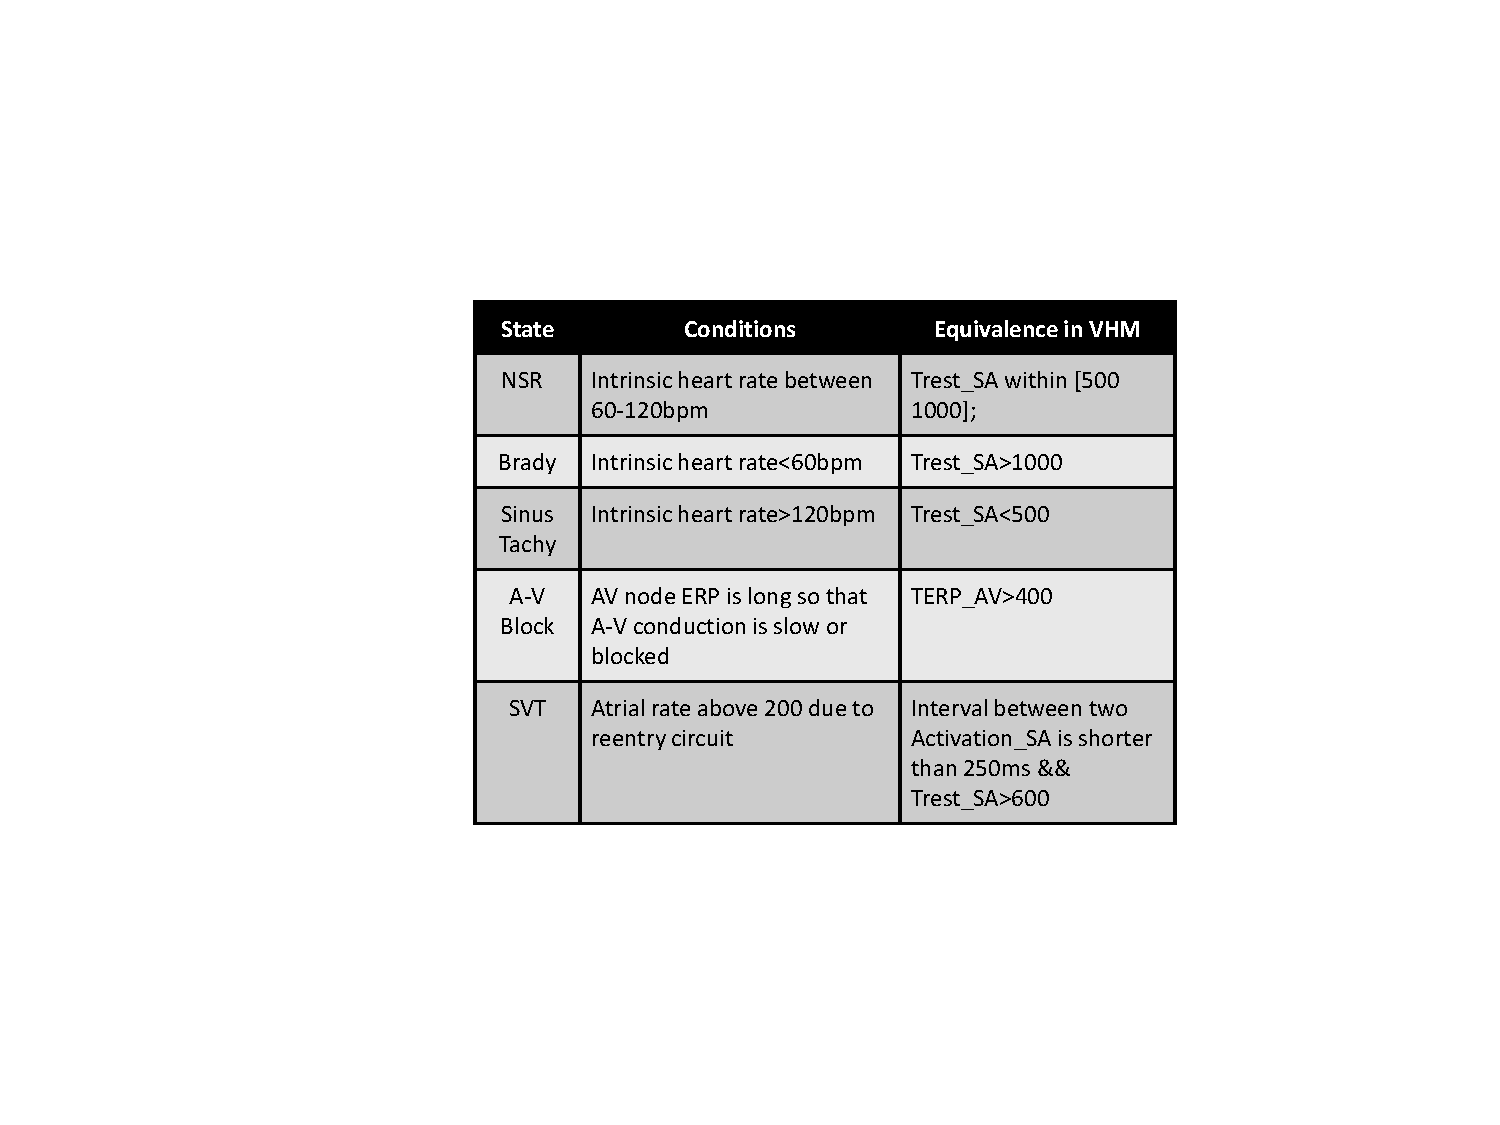
\includegraphics[width=0.70\textwidth]{figs/state.pdf}
	\center
	\vspace{-10pt}	
	\caption{Patient state and equivalence in the heart model}
	\vspace{-10pt}	
	\label{fig:state}
\end{figure}

\noindent
\textbf{2. Conditional Requirements:} Physiological requirements are in general conditional requirements. Specifying conditional requirements enables tighter constraints on the closed-loop system. \figref{conditional} shows a list of conditional requirements for normal sinus rhythm (NSR), supraventricular tachycardia (SVT), and bradycardia used during the pacemaker case study. 
\begin{figure}
	\center
	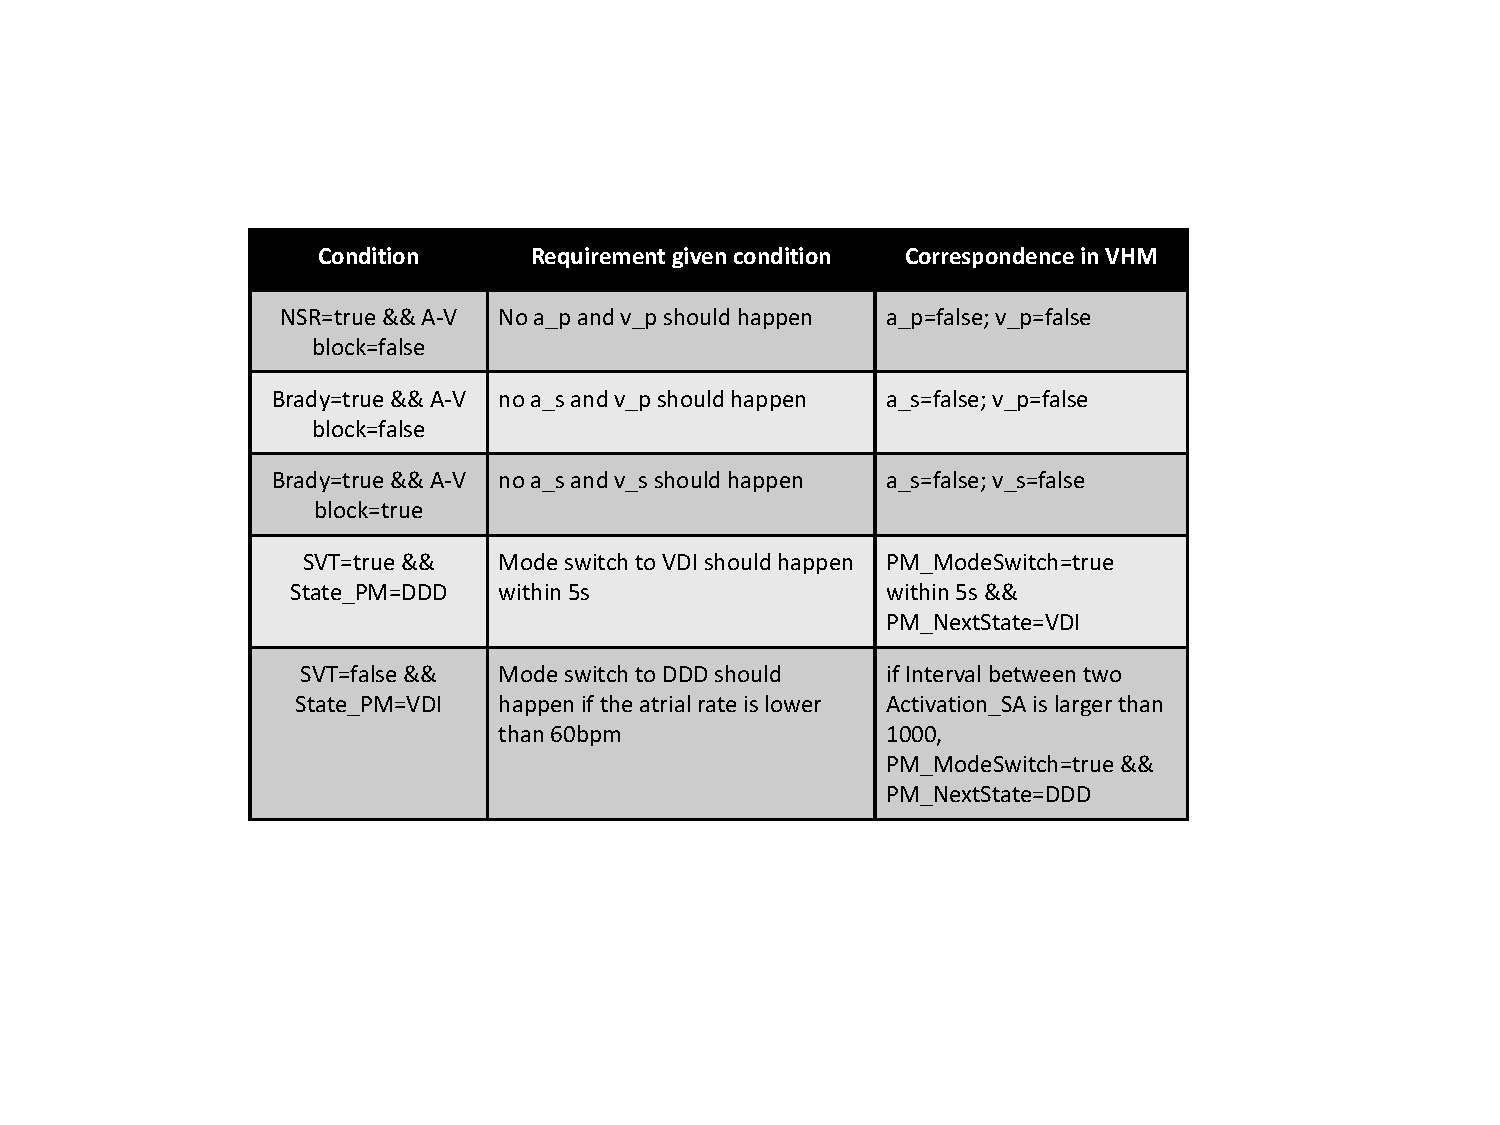
\includegraphics[width=0.7\textwidth]{figs/conditional.pdf}
	\center
	\vspace{-10pt}
	\caption{Conditional requirements for the close-loop system}
		%\vspace{-15pt}
	\label{fig:conditional}
\end{figure}
\begin{figure}
	\center
	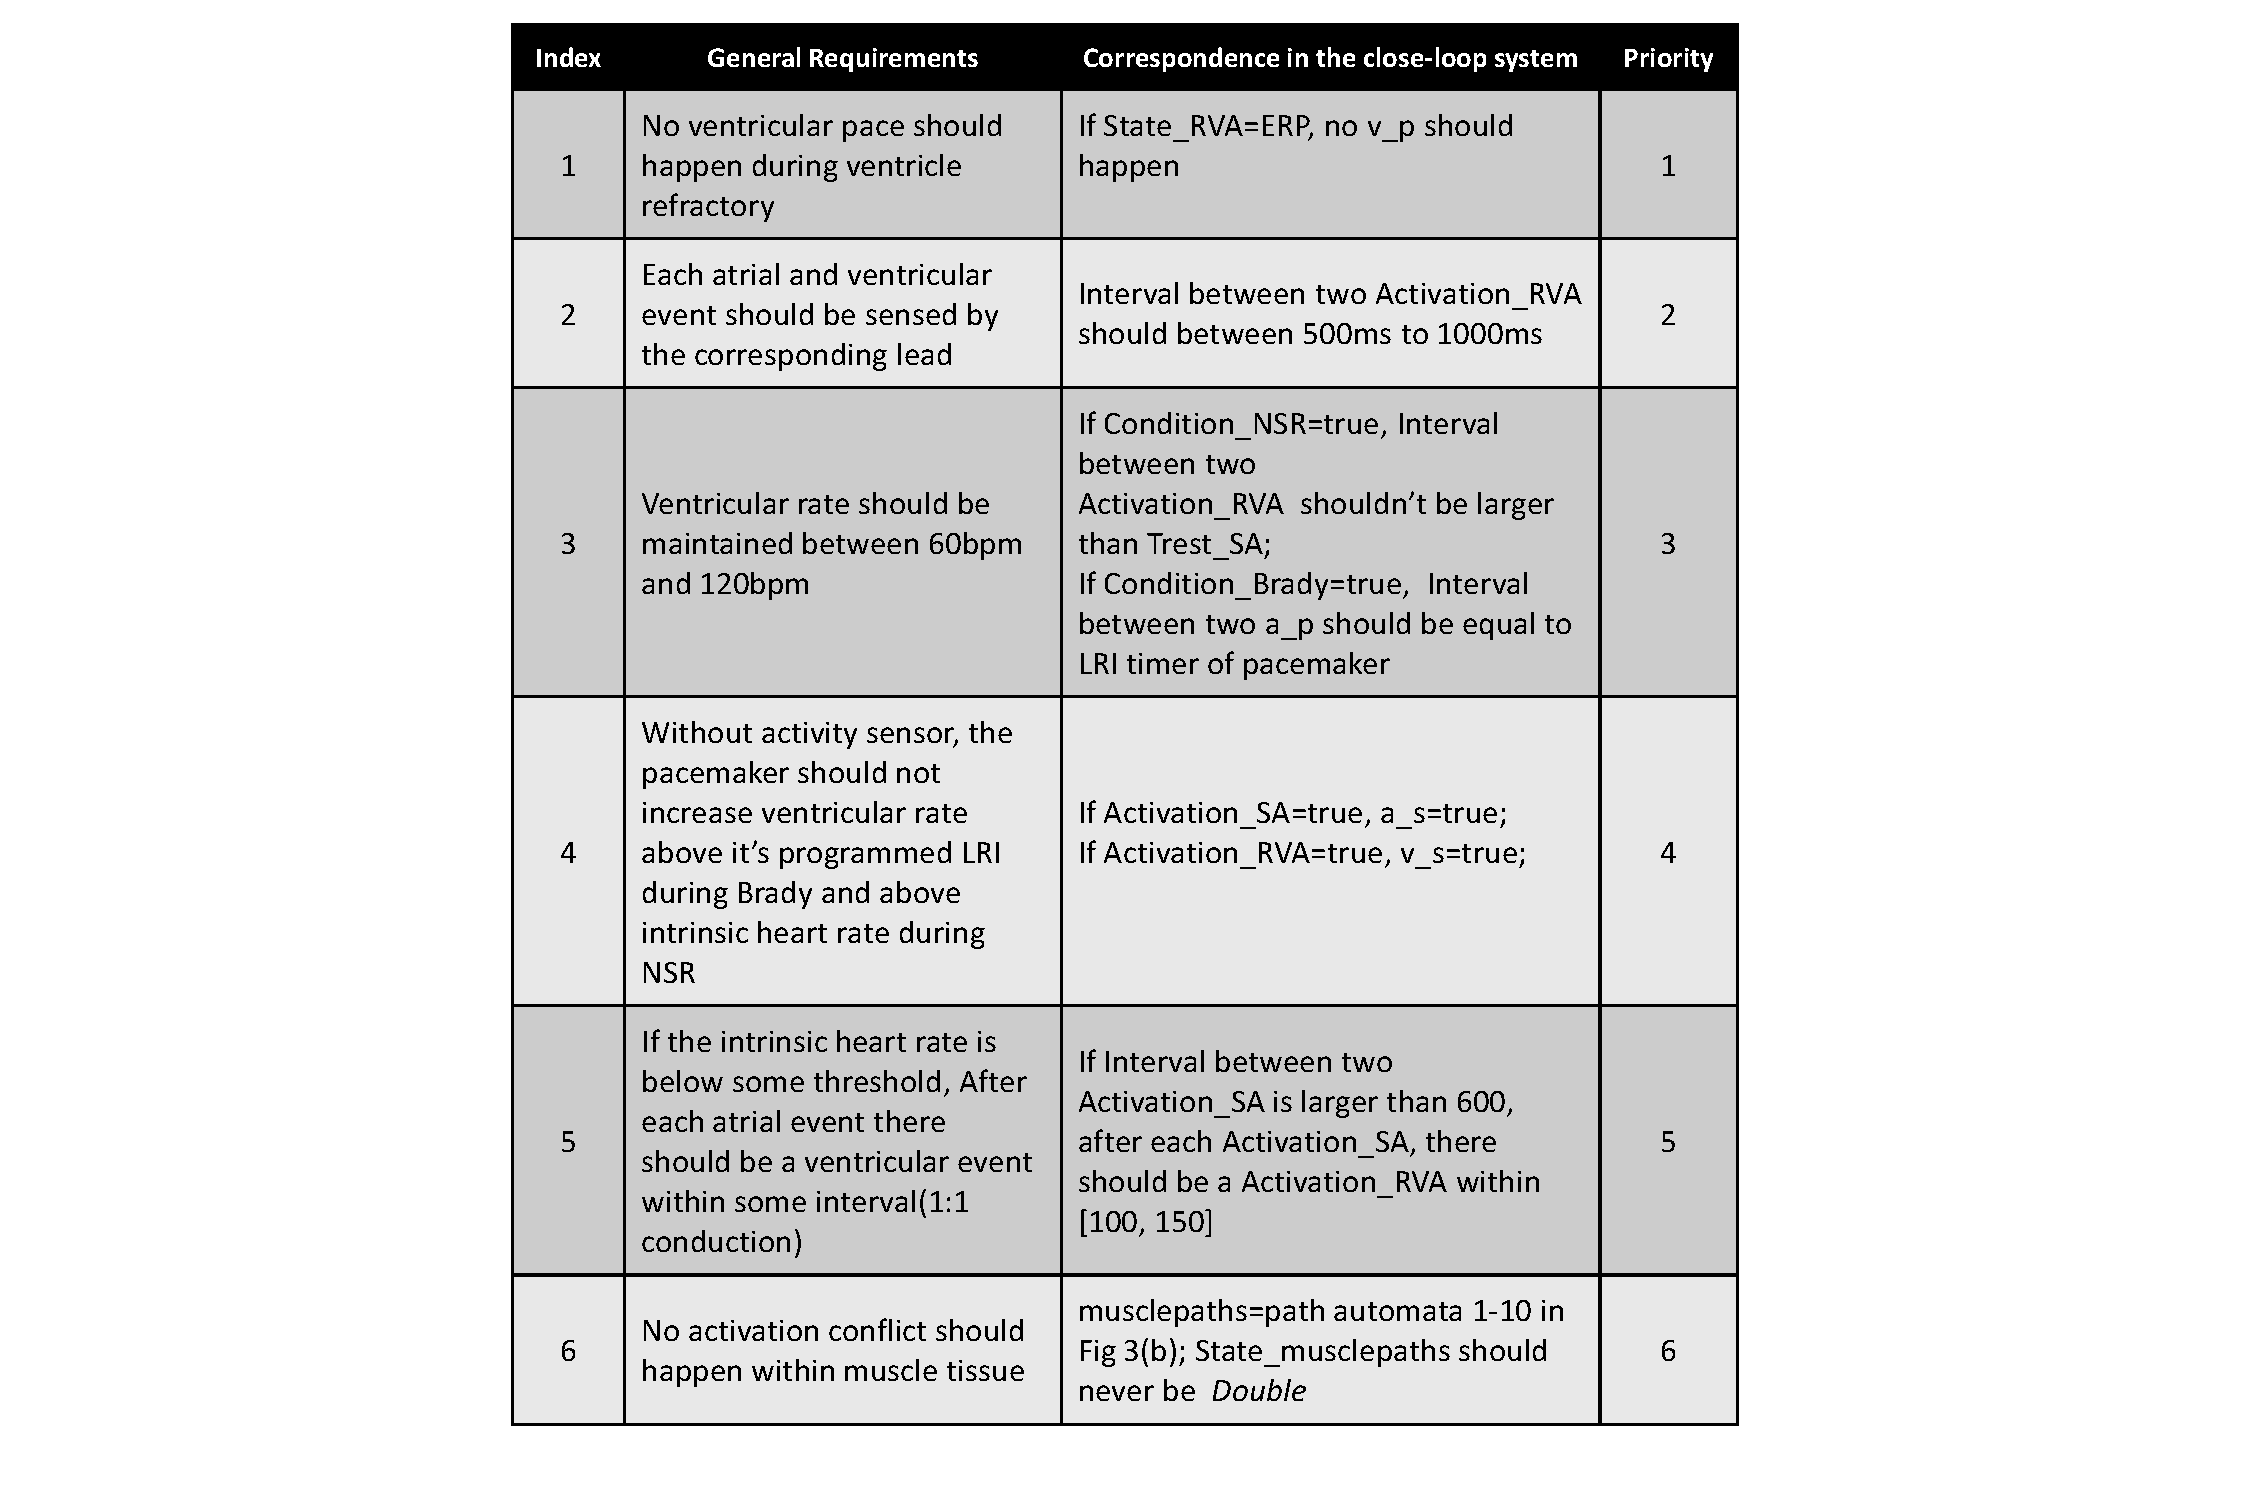
\includegraphics[width=0.7\textwidth]{figs/properties.pdf}
	\center
	\vspace{-10pt}
	\caption{General requirements for the close-loop system}
		%\vspace{-15pt}
	\label{fig:properties}
\end{figure}

\noindent
\textbf{3. Requirement Hierarchy}
For a closed-loop system including a heart $H$ and a pacemaker $P$: $S=H || P$ and two requirements $\varphi_1$ and $\varphi_2$ such that $\mathbb{P}_{\varphi_1}<\mathbb{P}_{\varphi_2}$, the following statement should always hold:
\vspace{-5pt}
$$H\models\varphi_2\rightarrow H||P\models\varphi_2$$
\noindent
meaning if a higher priority requirement is satisfied by the open-loop environment, it should be satisfied by the closed-loop system as well. An example violation of the statement is:
$$H\not\models\varphi_1 \&\& H\models\varphi_2 \&\& H||P\models\varphi_1 \&\& H||P\not\models\varphi_2$$
\noindent
which should not be allowed. In our closed-loop verification of pacemaker, the list of physiological requirements with assigned priorities are showing in \figref{properties}.





%\section{Requirement Representations}
%\subsection{TCTL}
%\subsection{Simulink Block}

